% 11-768 AI Agents, final project report (ACL format). Draft of 2026-11-27.
% Every number comes from the repository's result files (results/, commit 8c89308).
% Red [TODO: ...] marks parts the team still has to fill in. Remove \todo{} before submitting.
\pdfoutput=1
\documentclass[11pt]{article}
\usepackage{acl}
\usepackage{times}
\usepackage{latexsym}
\usepackage[T1]{fontenc}
\usepackage[utf8]{inputenc}
\usepackage{microtype}
\usepackage{inconsolata}
\usepackage{amsmath}
\usepackage{amssymb}
\usepackage{booktabs}
\usepackage{multirow}
\usepackage{graphicx}
\usepackage{xcolor}
\usepackage{xurl}
\usepackage{enumitem}

\newcommand{\todo}[1]{\textcolor{red}{[TODO: #1]}}
\newcommand{\iv}[2]{[$#1$,\,$#2$]}
\newcommand{\tsf}[1]{\textsc{#1}}

\setlist{nosep,leftmargin=*}

\title{Learning Scope-Aware Memory Revision for Evolving User Preferences}

% TODO: check names, order and spelling; add the third member.
\author{Zichu Wu \\ Carnegie Mellon University \And
  Raina Qiu \\ Carnegie Mellon University \And
  \todo{third member} \\ Carnegie Mellon University}

\begin{document}
\maketitle

\begin{abstract}
An assistant that remembers user preferences must decide, after each conversation, whether a statement changes the general preference, adds an exception that holds only in some situation or period, revises or retires such an exception, or changes nothing. We ask whether a memory manager trained to write an explicit scope-aware representation (records with a situation, a validity period and a link to the general preference they qualify) handles these cases better than one trained to write generic CRUD memory from the same evidence. We define an executable revision protocol in which both representations are projected from the same gold states, build a 920-episode synthetic chronological corpus and a hand-written challenge set, and fine-tune Qwen3-4B-Instruct-2507 with LoRA for each representation (three seeds); a frozen Answer Agent answers multiple-choice preference questions from each arm's own memory. Fine-tuning improves over prompting by 21--30 points in both arms. On the test split, evaluated once after all settings were frozen, the scope-aware arm leads (86.1\% vs.\ 83.3\%, $+2.7$ \iv{+0.9}{+4.5}), but the same gap appears when both arms hold gold memory, and the sign reverses on the development split. Re-reading the stored memories shows that the lead comes from how the reader uses the structured display rather than from better writing: rendered as CRUD sentences, the scope-aware memories score no better than CRUD memories. Both memories beat reading the raw conversation history by 25--28 points, and a larger reader preserves the test lead.
\end{abstract}

\section{Introduction}

LLM agents that talk with the same user over weeks increasingly keep an external memory of what the user prefers \citep{packer2023memgpt,chhikara2025mem0,xu2025amem}. Writing to that memory is a sequence of decisions: after each conversation, a memory manager decides what to add, change, delete or leave alone. Recent work learns these decisions, for example with reinforcement learning over ADD, UPDATE, DELETE and NOOP operations \citep{yan-etal-2026-memory,ma-etal-2026-fine}.

Preferences, however, rarely change by simple replacement. A user who usually wants an aisle seat may ask for a window seat on scenic journeys; someone who drinks black coffee may want green tea at the office for two weeks; and such an exception may later be revised or end. A memory manager that treats the statement as an update overwrites the general preference; one that ignores it loses the exception; and one that stores both as unstructured text leaves the reader to work out which record applies on a given date and occasion. Benchmarks show that agents often fail to notice that a memory is outdated \citep{chao2026stale,li2026horizonbench}, but they evaluate memory systems as wholes, so it remains unclear whether an explicit representation of scope helps an agent \emph{write} the right memory, \emph{read} it, or neither.

We ask: \textbf{can a memory manager trained to write an explicit scope-aware representation preserve evolving user preferences better than one trained to write generic CRUD memory, when both learn from the same evidence?} The scope-aware representation stores each preference as a record with a value, a situation (or \emph{general}), a validity period and typed links to the record it qualifies or replaces. Our project outline fixed two hypotheses. \textbf{H1}: after supervised fine-tuning (SFT) on identical evidence, the scope-aware system answers preference questions better than the CRUD system, in particular questions about scoped exceptions, without losing accuracy on general updates and stable preferences. \textbf{H2}: SFT improves over prompting in both representations. An optional reinforcement-learning stage (H3) was not run.

To keep the comparison controlled, both arms' training targets are projected from the same sequence of gold states, so the arms differ only in the representation they write (\S\ref{sec:method}). We build a 920-episode synthetic corpus audited for shortcut cues and a hand-written challenge set of structure-heavy cases (\S\ref{sec:data}). We fine-tune Qwen3-4B-Instruct-2507 \citep{yang2025qwen3} with LoRA \citep{hu2022lora} for each arm and three seeds, compare with zero- and six-shot prompting, and score both arms with the same frozen Answer Agent, bracketed by gold-memory and empty-memory references. All settings were frozen before the test split was evaluated, once. Our findings (\S\ref{sec:results}):
\begin{itemize}
\item SFT adds 21--30 points over prompting in both representations (H2 holds).
\item H1 holds on test ($+2.7$ points \iv{+0.9}{+4.5}; $+4.3$ on scoped-exception questions), but not on dev ($-2.5$) or the challenge set ($+0.4$).
\item The test lead equals the format gap on gold memory. Re-reading the stored memories in other displays attributes it to the structured display ($+3.2$), not to what the scope-aware policy writes ($-0.5$), also with a larger reader.
\item Both memories beat answering from the raw conversation history by 25--28 points.
\end{itemize}
In this controlled setting, explicit scope helps the reader more than the writer, and comparisons of memory designs should separate the two. Code, data and all result files are in our repository.\footnote{\url{https://github.com/kldxbjz/scope-aware-memory-revision} (private; access for course staff). This report uses commit \texttt{8c89308}.}

\section{Related Work}

\paragraph{Learned memory managers.} MemGPT \citep{packer2023memgpt} pages information between the context window and external storage, Mem0 \citep{chhikara2025mem0} extracts and consolidates salient facts, and A-Mem \citep{xu2025amem} links notes into an evolving network. Memory-R1 \citep{yan-etal-2026-memory} trains a Memory Manager that chooses ADD, UPDATE, DELETE or NOOP, together with an Answer Agent that selects and reasons over memory entries, using outcome-driven RL from only 152 QA pairs. Fine-Mem \citep{ma-etal-2026-fine} adds step-level rewards and evidence-anchored credit assignment for memory operations. Our CRUD arm adopts Memory-R1's operation set and its split into a memory manager and an Answer Agent, but trains the manager with SFT on projected gold operations; it is a Memory-R1-style baseline, not a reproduction. These systems store unscoped entries. We ask what changes when entries carry an explicit scope, validity and relations while supervision is held fixed.

\paragraph{Evolving preferences and stale memory.} PAMU \citep{sun-etal-2026-preference} fuses sliding-window and exponential moving averages into a preference representation that tracks short-term fluctuations and long-term tendencies; it models gradual drift, whereas we model discrete exceptions with explicit conditions. STALE \citep{chao2026stale} tests whether agents notice that a later observation implicitly invalidates an earlier memory and finds a wide gap between retrieving updated evidence and acting on it; its CUPMem prototype strengthens write-time revision through structured state consolidation, and StateAuditor \citep{sun2026stateauditor} repairs responses that still depend on stale state. HorizonBench \citep{li2026horizonbench} generates months of conversation in which preferences change after life events and finds that all evaluated models choose outdated preferences more often than chance would predict. PrefEval \citep{zhao2025prefeval}, LoCoMo \citep{maharana2024locomo} and LongMemEval \citep{wu2025longmemeval} test preference following, long conversational memory and knowledge updates. These benchmarks mostly involve global changes; our protocol targets the distinction between a general update and a situation- or time-limited exception, with every intermediate memory state exactly scorable.

\paragraph{Evaluating memory designs.} End-to-end QA mixes several parts of a memory system. LongMemEval splits memory into indexing, retrieval and reading, and shows that the reading stage affects accuracy even when the right evidence is available \citep{wu2025longmemeval}. MemDelta \citep{wang2026memdelta} varies one component at a time and finds that swapping the language or embedding model can reverse a comparison. Memory Tax \citep{he2026memorytax} measures the net value of memory against direct retrieval from the raw history and finds it is often negative. MAPE \citep{ding2026mape} identifies composing evidence for the answering model as a recurring trait of effective memory designs. MemSyco-Bench \citep{xiang2026memsyco} tests whether agents respect a memory's applicable scope and use only valid memories. We apply this lens to a write-time representation: gold-memory references and display swaps separate writing from reading, a raw-history condition measures the net value of memory, and a second reader tests reader dependence.

\section{Data}\label{sec:data}

\subsection{Task}
An episode describes one fictional user, one or two preference attributes (e.g., \emph{train seat}) with a catalogue of values and situations, and 4--8 dated events. Each event is a short conversation (3, 5 or 7 messages) between the user and an assistant. After every event, the gold state of each attribute is a general value plus a set of exceptions, each tied to a situation (e.g., \emph{scenic journeys}) and a validity: persistent, a dated window, or open (stated as temporary, with no end). Every event has exactly one of six categories (Table~\ref{tab:data}): a \emph{general update} changes the general value and keeps the exceptions; a \emph{scoped exception} adds one; an \emph{exception revision} changes an exception's value or validity; an \emph{exception retirement} removes one, so its situation inherits the general value again; a \emph{stable preference} event changes nothing (one-off requests, other people's preferences, hypotheticals, rejected suggestions, reaffirmations); and in a \emph{clarify} event the user leaves the change genuinely open, which the memory manager should flag rather than store.

After two to four events per episode, multiple-choice probes ask which value applies in a given situation on a given date (four options, chance 25\%). The gold answer is the value of the one exception whose situation and validity cover the probe, or else the general value. Probe types are \emph{target} (the situation that changed), \emph{default} (an ordinary occasion, where the general value holds), \emph{neighbor} (another situation of the same attribute) and \emph{boundary} (a date just outside a window). Probes are also grouped by the category of the event they follow (general update; scoped exception; exception revision, including retirements; stable preference, including clarifications).

\begin{table}[t]
\centering\small
\setlength{\tabcolsep}{4pt}
\begin{tabular}{@{}lrrrr@{}}
\toprule
 & Train & Dev & Test & Chall. \\
\midrule
Episodes & 600 & 120 & 200 & 24 \\
\quad with two attributes & 180 & 36 & 60 & 5 \\
Preference attributes & 28 & 28 & 28 & 29 \\
Events & 3,573 & 702 & 1,191 & 166 \\
\quad general update & 630 & 118 & 195 & 26 \\
\quad scoped exception & 683 & 107 & 211 & 32 \\
\quad exception revision & 605 & 171 & 227 & 31 \\
\quad exception retirement & 449 & 70 & 155 & 21 \\
\quad stable preference & 671 & 132 & 261 & 44 \\
\quad clarify & 535 & 104 & 142 & 12 \\
Probes & 6,011 & 1,170 & 2,027 & 567 \\
\quad target & 2,059 & 398 & 691 & 170 \\
\quad default & 1,541 & 320 & 531 & 124 \\
\quad neighbor & 2,103 & 424 & 717 & 253 \\
\quad boundary & 308 & 28 & 88 & 20 \\
\bottomrule
\end{tabular}
\caption{Data. Train, dev and test share no attribute, situation phrase or phrasing template; the hand-written challenge set shares no string with them.}
\label{tab:data}
\end{table}

\subsection{Synthetic corpus}
We found no public dataset with per-event labels that separate situation- or time-limited exceptions from general updates. We audited HorizonBench \citep{li2026horizonbench}, whose preference changes follow life events and apply globally; in the three users we inspected we could not confirm any observable scoped exception, so we did not use it and generated a corpus instead. A seeded, deterministic program composes timelines from split-specific banks of scenario families, phrasings and value aliases, which an LLM (GPT, through the Codex agent) authored under a written specification; every state change is sampled to be legal given the current state. The 84 attributes (one per scenario family) are split 28/28/28 with no shared attribute, situation phrase or template, so test measures transfer to new attributes. All content is fictional and in English.

A first release had strong shortcuts: a majority lookup by event position and number of stored exceptions predicted the category of 61\% of test events, and a bag-of-words classifier on the last user message 56\%. The released version randomises the event structure, diversifies the assistant's turns, lets users name attributes and values in their own words, and adds contrast pairs (episodes that differ in one earlier user message and have different gold transitions). On test the two shortcut classifiers fall to 28.9\% and 29.6\% (six classes), and no phrase confined to one category covers more than 15\% of its events. Every episode replays exactly through both arms' executors (\S\ref{sec:method}).

\paragraph{Label audit.} Because the labels come from a generator, we checked a sample before reading the test split: five events per category from train and from test (60 events) were shown with the stored preferences and the conversation but without labels, and one team member assigned a category to each. The annotator agreed with the generated category on 58 of 60 (Cohen's $\kappa=0.96$; \citealp{cohen1960kappa}); we checked the two disagreements against the category definitions (not blind) and kept the generated labels. A second team member's labels of the same events, recorded after the test run, agree with the first on 58 of 60 ($\kappa=0.96$) and with the generated categories on all 60; a third member adjudicated both disagreements for the generated labels. One annotator discussed some items with an AI assistant. No data changed.

\subsection{Challenge set}
The corpus has at most two exceptions per attribute and few long chains of changes. To test whether explicit structure matters more when cases need it, we wrote 24 episodes (166 events, 567 probes) under the same protocol, four for each of six stressors: \emph{dense} memory (3--4 exceptions per attribute), a situation \emph{shared} by two attributes, \emph{confusable} situations, order-dependent \emph{chains} of changes, \emph{temporal} windows that start later or end, and \emph{distractor} events about stored situations that must not change memory. The episodes were drafted with another LLM (Claude), independently of the corpus, and share no string with it. As a consistency check, two separate LLM instances that had not written the episodes labelled all 166 events blind; both agreed with every gold category. The evaluation plan was fixed before any model ran, including a data check on gold memory: the 25 probes that the Answer Agent missed in both arms were all reading errors, so no data changed.

\section{Method}\label{sec:method}

\subsection{Two memory representations}
Both arms keep a set of active records, which a memory manager (the \emph{policy}) edits once after every event through a deterministic executor. Figure~\ref{fig:example} shows the two formats.

\textbf{CRUD.} Records are free-text sentences with opaque ids. The policy returns operations ADD (text), UPDATE (id, text), DELETE (id) or a lone NOOP. Any number of records is allowed, so an exception can be stored as its own sentence, but nothing in the format marks which record is general.

\textbf{Scope-aware.} A record holds an attribute, a value, a scope (\texttt{general} or a situation phrase), a validity (persistent; a window with \emph{from} and \emph{to} dates; or open), relations, and the ids of the supporting events. An exception carries an \texttt{EXCEPTION\_TO} edge to the active general record of its attribute. The policy returns ADD, REVISE (a full new version of a target, which the executor links with \texttt{REPLACES} and retires), RETIRE (exceptions only) or NOOP. If any rule is broken (an unknown or inactive target, a second general record, an exception without its edge, evidence from an unseen event, a malformed field), the executor rejects the whole output and keeps the memory unchanged. Retired records stay in an audit log that the reader does not see.

In both arms the policy also returns a decision, \texttt{resolved} or \texttt{clarify}; a clarification comes with a single NOOP.

\begin{table}[t]
\centering\footnotesize
\setlength{\tabcolsep}{3pt}
\begin{tabular}{@{}lll@{}}
\toprule
Gold change & Scope-aware & CRUD \\
\midrule
General value & REVISE its record & UPDATE its record \\
New exception & ADD, linked & ADD \\
Exception changes & REVISE & UPDATE \\
Exception removed & RETIRE & DELETE \\
None, or clarify & NOOP & NOOP \\
\bottomrule
\end{tabular}
\caption{Fixed projection of gold state changes to each arm's training targets. A new scope-aware exception is linked to the general record by \texttt{EXCEPTION\_TO}.}
\label{tab:ops}
\end{table}

\subsection{Supervision from shared gold states}
For each training event, both arms' target outputs are computed from the gold states before and after it by the fixed mapping in Table~\ref{tab:ops}, never written by hand. CRUD sentences follow two templates (``For \emph{attribute}, the user prefers \emph{value}.'' and ``For \emph{attribute} when \emph{situation}, the user prefers \emph{value}.'', with the window or open validity appended). The policy's input is its arm's memory and the event (id, date and dialogue), byte-identical across arms apart from the memory, after a fixed instruction per arm that ends with one worked example on a made-up attribute (Appendix~\ref{app:prompts}). The arms thus see the same evidence and learn the same transitions; they differ in the representation they write and, as a consequence, in output length and in the rules the executor enforces.

Early gold writes used catalogue names that the policy often never saw, because in about half of the writes the user had used an alias. From protocol version 1.2 on, a gold write copies the user's own words; on dev this raised the share of written values in a listed form from 47--48\% to 96--97\% and accuracy by 1.5 (CRUD) and 2.1 (scope-aware) points. All results use version 1.2.

\subsection{Models and conditions}
Policies and the Answer Agent use Qwen3-4B-Instruct-2507 \citep{yang2025qwen3}, a non-thinking instruction model, with greedy decoding.

\textbf{Prompting (M0 CRUD, M1 scope-aware).} Zero-shot uses the instruction alone; six-shot adds one training event per category, the same six events for both arms, as earlier turns in each arm's format.

\textbf{SFT (M2 CRUD, M3 scope-aware).} We train one LoRA adapter \citep{hu2022lora} per arm and seed on the 3,573 training events: rank 16, $\alpha=32$, dropout 0.05 on all linear layers; learning rate $10^{-4}$ with cosine decay and 3\% warm-up; 2 epochs at batch size 16 (4 with 4 accumulation steps), i.e.\ 448 steps; loss on the completion only; bf16; TRL 0.24 \citep{vonwerra2020trl} and PEFT 0.17 \citep{mangrulkar2022peft}. No example is truncated. No hyperparameter was tuned on dev; we use the final checkpoints of seeds 0, 1 and 2.

\textbf{References.} \emph{Gold memory} gives the Answer Agent each arm's gold memory after every event, its ceiling with correct memory; \emph{never written} gives it the initial memory only, the floor. The two arms' gold memories hold the same content, so their difference measures the format alone.

\subsection{Rollout, Answer Agent and metrics}
Episodes are replayed in date order. At each event the policy sees only that event and its own current memory and writes up to 512 tokens; the executor applies the output, and a rejected output leaves the memory as it was. Each probe reads the active memory after its event.

The Answer Agent is the base model without any adapter, the same for both arms. Its prompt lists the memory records as JSON, the date, the question and the options, adds one reading rule (a record limited to a situation or to dates applies only there and then; otherwise the general preference holds), and asks for a one-sentence check and a final ``Answer:'' line (at most 160 tokens; Appendix~\ref{app:prompts}). We chose this prompt among three versions on dev gold memory alone, before any SFT result existed (mean gold-memory accuracy 89.9, 91.4 and 92.9\%).

The primary metric is Answer Agent accuracy on each arm's own rollout memory; for SFT, a probe scores the share of the three seeds that answered it correctly. H1 is SFT scope-aware minus SFT CRUD; H2 is SFT minus each prompt baseline. Intervals are 95\% percentile bootstraps over episodes (one fictional user each, with all its probes and seeds; 2,000 resamples, paired across arms; \citealp{efron1993bootstrap}). To see how far a result carries over to new attributes, we also resample the 28 attributes (\emph{family} intervals). Boundary probes are few, and even gold memory fails most of them, so we also report results without them. Write-level metrics from deterministic rule readers serve as diagnostics only.

\textbf{Protocol.} Dev served all development decisions. All settings were frozen (a git tag) after the challenge-set runs and the label audit, and the test split was then evaluated once. Analyses added afterwards re-read the stored test memories and are marked \emph{post-hoc}; they do not replace the main table.

\textbf{Compute.} Runs used single GPUs (A100, A6000, L40, L40S, RTX 6000 Ada) of a university cluster, at no monetary cost; one SFT run takes 0.5 (CRUD) to 1.5 (scope-aware) hours, and the seven test runs took 8.2 GPU-hours.

\begin{figure*}[t]
\centering\small
\fbox{\begin{minipage}{0.975\textwidth}
\textbf{Question} (test episode te-0114, dated 2 August): \emph{Pick a value for stylus pressure response, dated August 2, with the setting described as an ordinary occasion.}\quad
\textbf{Options:} a gradual midrange pressure curve $|$ a light-touch pressure curve $|$ a nearly uniform stroke response $|$ \underline{a firm-pressure response curve} (gold)
\end{minipage}}\\[5pt]
\begin{minipage}[t]{0.485\textwidth}\raggedright
\textbf{CRUD memory}\\[2pt]
{\footnotesize\ttfamily \{"id": "m1", "text": "For stylus pressure response, the user prefers a firm-pressure response curve."\}\\
\{"id": "m2", "text": "For stylus pressure response when stylus work on a textured screen cover, the user prefers a nearly uniform stroke response."\}}\\[4pt]
\textbf{Answer Agent} ($\times$): \emph{The record that applies on this date and in this situation is m2, which describes a nearly uniform stroke response when working on a textured screen cover. Answer: a nearly uniform stroke response}
\end{minipage}\hfill
\begin{minipage}[t]{0.485\textwidth}\raggedright
\textbf{Scope-aware memory} (attribute and evidence ids not shown)\\[2pt]
{\footnotesize\ttfamily \{"memory\_id": "m1", "value": "a firm-pressure response curve", "scope": "general", "validity": \{"kind": "persistent"\}, "relations": []\}\\
\{"memory\_id": "m2", "value": "a nearly uniform stroke response", "scope": "stylus work on a textured screen cover", "validity": \{"kind": "persistent"\}, "relations": [\{"type": "EXCEPTION\_TO", "target": "m1"\}]\}}\\[4pt]
\textbf{Answer Agent} ($\checkmark$): \emph{The general record (m1) applies on this date and in this situation, as the scenario describes an ordinary occasion without specifying a textured screen cover. Answer: a firm-pressure response curve}
\end{minipage}
\caption{The same content in the two formats (test, SFT seed 0; both memories still hold the episode's two initial records). The 4B Answer Agent applies the situation-specific CRUD sentence to an ordinary occasion, but picks the general record from the scope-aware display. On the 531 test questions about ordinary occasions it answers 79.7\% correctly from SFT CRUD memory and 91.0\% from SFT scope-aware memory.}
\label{fig:example}
\end{figure*}

\section{Results}\label{sec:results}

\subsection{Main result on test}

\begin{table}[t]
\centering\small
\setlength{\tabcolsep}{3.5pt}
\begin{tabular}{@{}lccc@{}}
\toprule
Condition & CRUD & Scope & Scope $-$ CRUD \\
\midrule
Never written & 48.1 & 50.1 & $+2.0$ \iv{+1.0}{+3.0} \\
Zero-shot & 56.6 & 57.0 & $+0.4$ \iv{-2.9}{+3.7} \\
Six-shot & 53.8 & 65.3 & $+11.5$ \iv{+8.1}{+14.9} \\
SFT, 3 seeds & \textbf{83.3} & \textbf{86.1} & $\mathbf{+2.7}$ \iv{+0.9}{+4.5} \\
Gold memory & 86.9 & 89.6 & $+2.7$ \iv{+1.2}{+4.2} \\
\bottomrule
\end{tabular}
\caption{Test results: Answer Agent accuracy (\%) on 2,027 probes per arm, with 95\% episode-bootstrap intervals; evaluated once with frozen settings. Without the 88 boundary probes, scope $-$ CRUD is $+1.7$ \iv{-0.2}{+3.4} after SFT and $+1.7$ \iv{+0.1}{+3.1} on gold memory.}
\label{tab:main}
\end{table}

\paragraph{H2 holds.} SFT raises accuracy by 26.7 (over zero-shot) and 29.6 (over six-shot) points for CRUD and by 29.0 and 20.8 points for the scope-aware arm (Table~\ref{tab:main}); every interval is far from zero. In both arms SFT closes about 91\% of the gap between never-written and gold memory. The prompted scope-aware policy often breaks the executor's rules (on dev mostly an ADD without a valid attribute or a REVISE without its target): 312 of 1,191 zero-shot and 371 six-shot outputs are rejected (CRUD: 5 and 13). After SFT, 11 of 3,573 scope-aware outputs are rejected and no CRUD output.

\paragraph{H1 holds on test.} After SFT the scope-aware arm answers 86.1\% against 83.3\%, $+2.7$ \iv{+0.9}{+4.5}; without boundary probes $+1.7$ \iv{-0.2}{+3.4}. All three seeds point the same way ($+2.8$, $+0.8$, $+4.5$). On scoped-exception questions, which H1 singles out, the difference is $+4.3$ \iv{+1.5}{+7.0}, and the other groups do not get worse (general update $+0.7$, exception revision $+2.8$, stable preference $+2.1$; all intervals include zero).

\paragraph{But gold memory shows the same gap.} With gold memory in both arms, i.e.\ the same content in the two formats, the scope-aware format is read 2.7 points better \iv{+1.2}{+4.2}. The pattern across question types matches the SFT difference almost exactly (Figure~\ref{fig:types}): large gains on default ($+11.2$ after SFT, $+11.1$ on gold) and boundary questions ($+25.8$, $+26.1$), small losses on target ($-2.4$, $-1.6$) and neighbor questions ($-1.4$, $-2.2$), and on scoped-exception questions $+4.3$ against $+4.5$.

\begin{figure}[t]
\centering
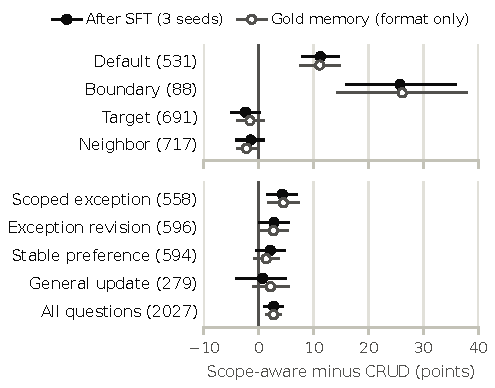
\includegraphics[width=\columnwidth]{figures/report_fig_types.pdf}
\caption{Scope-aware minus CRUD on test by question type (top) and question group (bottom), after SFT and on gold memory, with 95\% episode-bootstrap intervals; probes in brackets. The two patterns coincide.}
\label{fig:types}
\end{figure}

\subsection{Three episode sets, three answers}

\begin{table*}[t]
\centering\small
\setlength{\tabcolsep}{4pt}
\begin{tabular}{@{}lcccccl@{}}
\toprule
 & \multicolumn{2}{c}{SFT accuracy} & \multicolumn{3}{c}{Scope $-$ CRUD (points)} & \\
\cmidrule(lr){2-3}\cmidrule(lr){4-6}
Episode set & CRUD & Scope & Total, after SFT & Format (gold memory) & Writing & Per seed (total) \\
\midrule
Dev & 88.8 & 86.3 & $-2.5$ \iv{-5.2}{+0.3} & $+0.1$ \iv{-2.4}{+2.5} & $-2.5$ \iv{-4.3}{-1.0} & all three $<0$ \\
Test & 83.3 & 86.1 & $+2.7$ \iv{+0.9}{+4.5} & $+2.7$ \iv{+1.2}{+4.2} & $+0.0$ \iv{-1.5}{+1.3} & $+2.8$, $+0.8$, $+4.5$ \\
Challenge & 80.6 & 81.0 & $+0.4$ \iv{-2.9}{+4.0} & $+1.2$ \iv{-2.6}{+4.9} & $-0.8$ \iv{-4.8}{+3.4} & $+6.7$, $-2.8$, $-2.6$ \\
\bottomrule
\end{tabular}
\caption{The SFT difference on dev (120 episodes, 1,170 probes), test (200, 2,027) and the challenge set (24, 567), split into format (the gap on gold memory) and writing (how much less the scope-aware policy loses against its own gold memory than the CRUD policy); total = format + writing. The split is post-hoc; for the challenge set it was computed for this report.}
\label{tab:sets}
\end{table*}

The test result did not appear on the other two sets (Table~\ref{tab:sets}). On dev the scope-aware arm trailed ($-2.5$ \iv{-5.2}{+0.3}, all seeds below zero); on the challenge set the arms tied ($+0.4$ \iv{-2.9}{+4.0}) and the seeds disagreed. No challenge stressor favoured the scope-aware arm except \emph{chain} ($+7.3$), which one episode drives (Appendix~\ref{app:extra}). The three sets use disjoint attributes, and the difference varies strongly between attributes (Figure~\ref{fig:attributes}): from $-33.3$ to $+12.8$ points on dev (SD 10.3; scope-aware ahead on 9 of 28) and from $-9.9$ to $+13.2$ on test (SD 4.9; ahead on 20 of 28). The splits' mixes of question types explain little: reweighted to test's mix, dev still gives $-1.8$ \iv{-4.7}{+1.0}.

\subsection{Writing or reading?}\label{sec:readwrite}

\paragraph{Decomposition (post-hoc).} We split each SFT difference into a \emph{format} part, the gap on gold memory, and a \emph{writing} part, $(\text{SFT}_{s}-\text{gold}_{s})-(\text{SFT}_{c}-\text{gold}_{c})$. On test the whole lead is format: writing contributes $+0.0$ \iv{-1.5}{+1.3} (family interval \iv{-1.9}{+1.6}). On dev the deficit is writing, $-2.5$ \iv{-4.3}{-1.0}, with format $+0.1$; on the challenge set both parts are near zero (Table~\ref{tab:sets}). Teacher-forced write metrics, where each output is applied to the gold memory before its event, agree (Appendix~\ref{app:extra}): on test both policies handle about 91\% of events exactly right (CRUD 91.7, scope-aware 91.2), while on dev the scope-aware policy is 2.4 points behind, mostly on new scoped exceptions (84.7\% against 94.4\%). It also misses more of the events that call for clarification (96.2\% against 99.3\% handled on test).

\paragraph{Display experiment (post-hoc).} The decomposition rests on gold memory. To measure the format effect on the memories the policies actually wrote, we re-read every stored scope-aware SFT memory in three displays: \emph{replay}, the original prompt answered again; \emph{CRUD sentences}, every record rendered with the CRUD arm's templates, so that the content is the scope-aware policy's and the display is CRUD's; and \emph{compact}, one block per attribute with the general value and one line per situation and its dates, without ids, relations or evidence. Nothing is repaired or dropped. Replays give the stored answer on 99.7\% of probes. Rendered as CRUD sentences, the scope-aware memories score 82.8\%, no better than the CRUD arm's own memories (83.3\%): the content part is $-0.5$ \iv{-2.2}{+1.1} and the display part $+3.2$ \iv{+1.9}{+4.5} (Table~\ref{tab:reader}). The display gains sit in default ($+10.0$) and boundary questions ($+18.9$), where an explicit general record and explicit validity fields tell the reader which record applies (Figure~\ref{fig:example}). The compact display cuts the memory block from 315 to 58 tokens but costs 3.0 points with this reader.

\subsection{Is a memory needed at all? (post-hoc)}
Our episodes are short (at most eight events), so an agent could simply re-read the conversations. In condition A the same Answer Agent answers each probe from the initial preferences and every conversation up to the probe, with the reading rule adapted to conversations. It scores 58.2\% \iv{55.7}{60.6} on test, 25.2 and 27.9 points below the SFT CRUD and scope-aware memories and only 8--10 points above never-written memory (dev: 35--38 points below). It does worst on ordinary occasions (48.0\%), where it applies a situation's or a temporary preference. Per seed, the memories answer 620--677 test probes that the history misses and miss 89--124 that it answers. A test run costs 1.55M tokens with the history and 1.40M (CRUD) or 2.17M (scope-aware) with memory, counting every write call.

\begin{table*}[t]
\centering\footnotesize
\setlength{\tabcolsep}{3pt}
\begin{tabular}{@{}lcccccc@{}}
\toprule
 & \multicolumn{2}{c}{Test (2,027 probes)} & \multicolumn{2}{c}{Dev (1,170)} & \multicolumn{2}{c}{Challenge (567)} \\
\cmidrule(lr){2-3}\cmidrule(lr){4-5}\cmidrule(lr){6-7}
Reader & 4B & 30B-A3B & 4B & 30B-A3B & 4B & 30B-A3B \\
\midrule
SFT CRUD memory & 83.3 & 81.9 & 88.8 & 85.4 & 80.6 & 83.3 \\
SFT scope-aware memory & 86.1 & 85.1 & 86.3 & 86.1 & 81.0 & 82.2 \\
Scope $-$ CRUD, SFT & $+2.7$ \iv{+0.9}{+4.5} & $+3.2$ \iv{+1.1}{+5.0} & $-2.5$ & $+0.7$ & $+0.4$ & $-1.1$ \\
Scope $-$ CRUD, gold memory & $+2.7$ \iv{+1.2}{+4.2} & $+3.5$ \iv{+1.6}{+5.3} & $+0.1$ & $+2.6$ & $+1.2$ & $+0.2$ \\
\midrule
A: raw history, no memory & 58.2 & 57.5 & 50.8 & 50.9 & & \\
\quad history $-$ SFT CRUD & $-25.2$ \iv{-28.0}{-22.4} & $-24.4$ \iv{-27.4}{-21.6} & $-37.9$ & $-34.4$ & & \\
\quad history $-$ SFT scope-aware & $-27.9$ \iv{-30.4}{-25.4} & $-27.6$ \iv{-30.4}{-24.9} & $-35.5$ & $-35.2$ & & \\
\midrule
B: display part (original $-$ sentences) & $+3.2$ \iv{+1.9}{+4.5} & $+3.6$ \iv{+2.0}{+5.1} & $+2.0$ & $+2.6$ & & \\
\quad content part (sentences $-$ CRUD) & $-0.5$ \iv{-2.2}{+1.1} & $-0.4$ \iv{-2.0}{+1.0} & $-4.4$ & $-1.8$ & & \\
\quad compact $-$ replay & $-3.0$ \iv{-4.3}{-1.6} & $+0.1$ \iv{-1.5}{+1.6} & $-2.2$ & $+1.4$ & & \\
\bottomrule
\end{tabular}
\caption{Robustness to the reader (post-hoc): the stored memories re-read by Qwen3-30B-A3B-Instruct-2507, with nothing else changed. B shows the scope-aware SFT memories in other displays; display part + content part = scope $-$ CRUD. The challenge set has no A or B runs. Dev intervals and B on gold memory are in the repository.}
\label{tab:reader}
\end{table*}

\subsection{Robustness to the reader (post-hoc)}
All results so far use one 4B reader. We re-read every stored dev, test and challenge memory, and repeated A and B, with Qwen3-30B-A3B-Instruct-2507 (30.5B parameters, 3.3B active), changing nothing else (Table~\ref{tab:reader}); the rules for judging the outcome were fixed before these runs. Three readings hold: the raw history stays 24--28 points below both memories on test (57.5\%); the display part stays positive ($+3.6$ \iv{+2.0}{+5.1} on test, $+2.6$ on dev) while the content part does not ($-0.4$); and the test lead stays, $+3.2$ \iv{+1.1}{+5.0} (family interval \iv{+1.1}{+5.5}). One does not: with the larger reader the compact display costs nothing ($+0.1$ on test, $+1.4$ on dev), so its cost was a property of the small reader.

The larger reader also moves the dev difference from $-2.5$ to $+0.7$ (n.s.), because it misreads CRUD memory on ordinary occasions, applying a situation's preference that is in effect on the probe's date (dev SFT CRUD accuracy on default questions: 84.2 $\rightarrow$ 68.0\%). On test this misreading hits both memories (CRUD 79.7 $\rightarrow$ 69.1\%, scope-aware 91.0 $\rightarrow$ 78.1\%); the lead grows slightly only because the scope-aware arm's small deficits on target and neighbor questions shrink and its boundary advantage grows. On the challenge set the arms still tie ($-1.1$ \iv{-4.2}{+1.8}).

\subsection{Error analysis}

\paragraph{Write errors.} At the test probes, the rule readers find the probed attribute's memory equal to the gold state for 84.2\% (CRUD) and 83.5\% (scope-aware) of probe-seed pairs. Where the scope-aware memory matches gold, its arm leads by 5.2 points \iv{+3.7}{+6.8}; where it holds a wrong value or structure, it trails by 16.6 and 11.2 points. Under teacher forcing both arms make the same kinds of errors (counts over three seeds, CRUD/scope-aware): skipping a new scoped exception (26/27), overwriting another record with it (20/11), turning an exception revision into a NOOP or a new record (38/40), and writing on stable-preference events (24/18).

\paragraph{Read errors.} Even with gold memory the 4B reader misses 10--13\% of test probes. Of the 25 challenge-set probes it missed on gold memory in both arms, 8 read a date outside a window as inside, 12 applied a situation record where the general value holds, and 5 did not match a record in the user's words to the question. Replies can also contradict themselves: one test reply states that the general preference applies and then answers with the exception's value.

\paragraph{Manual attribution.} \todo{Report the settled labels here once the two annotators finish.} The pre-specified packets hold 40 randomly drawn wrong probes per arm (SFT seed 0; 275 scope-aware and 332 CRUD wrong probes in all). Each is labelled by two annotators with the first applicable source: data, executor rejection, action (a wrong or missing write), reader matching, answer reasoning, or other (Appendix~\ref{app:manual}).

\paragraph{Cost.} Per event the scope-aware policy reads 884 and writes 65 tokens (CRUD 603 and 36), and per probe the reader reads 461 tokens (CRUD 263): a scope-aware memory takes 248 tokens at a probe, a CRUD memory 107.

\section{Discussion}

\paragraph{What the scope-aware representation buys.} Our evidence places its benefit at read time. Marking one record as \texttt{general} and giving every exception an explicit situation and validity makes two judgments easy for the reader: an ordinary occasion falls under the general record, and a window that has ended no longer applies. From CRUD sentences the reader must infer both from wording, and it often applies a situation-specific sentence to an ordinary occasion. On target and neighbor questions the structured display is slightly worse; we did not test why.

\paragraph{What it does not buy.} We expected explicit structure to make exceptions easier to learn and to keep apart from the general preference. It did not: after SFT both policies write about equally well on test, and on dev the scope-aware policy was worse at adding new scoped exceptions. The richer format adds failure modes (longer outputs, executor rules, missed clarifications) that SFT must also learn, and with 3,573 examples it learns the simpler CRUD format at least as well. Without SFT, the structured format is much harder to produce at all (up to 31\% of prompted outputs rejected).

\paragraph{Why the sign changes.} The end-to-end difference is the sum of a reading effect, which depends on the question mix and on the reader, and a writing effect, which varies with the attributes. Both vary across our three disjoint attribute samples, so the sign of H1 changes while the pattern by question type stays. As \citet{wang2026memdelta} observe for memory evaluation in general, the comparison is fragile: changing the reader moved the dev result by three points and removed the compact display's cost.

\paragraph{Implications for building agents.} With a fixed reader, a structured display of memory may be a cheaper lever than a structured write protocol: the display effect appears with both readers, the write effect with neither. Before a gain is attributed to the representation an agent writes, designs should be compared with gold-memory references, with displays swapped between arms, against a raw-history baseline, and with more than one reader.

\paragraph{Unexpected behaviour.} Our first run of the larger reader on two GPUs returned garbage: direct GPU-to-GPU copies on the cluster's nodes corrupted data although the driver reported peer access, and copying through host memory fixed it (Appendix~\ref{app:bigreader}). Such failures can look like model behaviour.

\section{Conclusion and Future Work}
With identical evidence and supervision, a 4B model learns to revise a preference memory well in both a generic CRUD and an explicit scope-aware representation; SFT adds 21--30 points over prompting. The scope-aware system answers 2.7 points more test questions, but its advantage is that of a structured display for the reader, not of better writing, and the sign of the end-to-end comparison depends on the attribute sample and on the reader. Beyond our setup, this suggests that memory representations should be evaluated separately for writing and for reading.

Useful next steps are a common structured display for both arms (which requires parsing CRUD sentences), read-time diagnostics on MemSyco-Bench's scope-control and valid-memory tasks \citep{xiang2026memsyco}, human-written conversations with longer timelines and overlapping situations, learning curves, and RL from the SFT checkpoints (H3) against a continued-SFT control.

\section*{Limitations}
\begin{itemize}
\item \textbf{Synthetic data.} Train, dev and test are generated from LLM-authored banks with 84 attributes, and the challenge set was drafted by another LLM. Conversations are short, timelines have at most eight events and two attributes, every event changes at most one record, situations never overlap, and each new value or situation is named in a listed form. Results may not transfer to real conversations.
\item \textbf{One model family.} The policy and both readers are Qwen3 models; the 4B reader shares its base model with the policies.
\item \textbf{Reader and metric.} QA is multiple choice with one prompt chosen on dev gold memory. The reader misses 10--13\% of probes even with gold memory, and boundary questions are few (88 on test).
\item \textbf{Sample size.} Each split has 28 attributes, between which the difference varies strongly; three seeds per arm.
\item \textbf{Post-hoc analyses.} The decomposition, display, raw-history and larger-reader analyses were added after the single test run. We fixed their reading rules before running them, but they are exploratory.
\item \textbf{Label checks.} The category audit covers 60 events and checks categories, not every value, date or probe; one annotator consulted an AI assistant; the challenge-set check used LLM annotators.
\end{itemize}

\section*{Ethical Considerations}
Preference memory is personal data. A scope-aware memory records not only what a user likes but in which situations and periods, a more detailed profile than a list of facts, which raises the stakes of leaks, secondary use such as targeting, and retention. Deployments should let users inspect, correct and delete records, including the audit log of retired records; explicit records make this easier. Misapplied memory can also harm users, for example when a temporary exception is applied permanently; our readers make such errors even with correct memory. Our data are fictional, contain no personal information and cover English everyday preferences only, so they support no conclusion about fairness across languages or groups.

\section*{Team Member Contributions}
\todo{Each member describes their own contributions (implementation, experiments, analysis, writing), e.g.\ the protocol, training and evaluation code; the label-audit annotations and adjudication; the mid-project update that proposed experiments A and B.}
\textbf{Zichu Wu}: \todo{...} \textbf{Raina Qiu}: \todo{...} \textbf{\todo{third member}}: \todo{...}

\paragraph{Use of AI tools.} \todo{Confirm this wording.} The corpus banks were authored with GPT (Codex) and the challenge set was drafted with Claude, whose separate instances also checked its labels. AI coding assistants helped write the code, run the experiments and draft this report. All numbers come from the result files in the repository, and every citation was checked against its source.

\bibliography{custom}

\appendix

\section{Prompts}\label{app:prompts}

\paragraph{Policy instructions.} The policy receives its arm's instruction as the system message and, as the user message, a JSON object with the memory and the event. The instructions, verbatim:

{\scriptsize\ttfamily\raggedright
\textbf{Scope-aware.} You maintain a user's long-term preference memory. Read the memory and the new conversation and return one JSON object \{"decision": "resolved" or "clarify", "actions": [...]\}. Records have memory\_id, attribute, value, scope ("general" or a situation), validity, relations and evidence\_ids. Actions: ADD \{operation, attribute, value, scope, validity, relations, evidence\_ids\}; REVISE \{operation, target\_id, value, scope, validity, relations, evidence\_ids\}, which replaces target\_id; RETIRE \{operation, target\_id, evidence\_ids\}, which removes a situation-specific record so that situation follows the general preference again; NOOP \{operation\}, alone. Validity is \{"kind": "persistent"\}, \{"kind": "window", "from": "YYYY-MM-DD", "to": "YYYY-MM-DD"\} or \{"kind": "open"\}. A situation-specific record needs relations [\{"type": "EXCEPTION\_TO", "target": <id of the general record>\}]. evidence\_ids name the event that supports the write. Store only lasting preferences of the user; one-off requests and other people's preferences need NOOP. If the user has not settled what should change, answer "clarify" with a single NOOP. Each action is an object whose "operation" field names it.\\
Example: the memory holds m1, the general drink order "black coffee", and the new conversation (event\_id "e9") says the user wants green tea at the office from 2030-03-01 through 2030-03-14. Output:\\
\{"actions": [\{"attribute": "drink order", "evidence\_ids": ["e9"], "operation": "ADD", "relations": [\{"target": "m1", "type": "EXCEPTION\_TO"\}], "scope": "at the office", "validity": \{"from": "2030-03-01", "kind": "window", "to": "2030-03-14"\}, "value": "green tea"\}], "decision": "resolved"\}\\
Nothing to store:\\
\{"actions": [\{"operation": "NOOP"\}], "decision": "resolved"\}\par
\medskip
\textbf{CRUD.} You maintain a user's long-term preference memory as free-text records. Read the memory and the new conversation and return one JSON object \{"decision": "resolved" or "clarify", "operations": [...]\}. Operations: ADD \{op, text\}; UPDATE \{op, id, text\}; DELETE \{op, id\}; NOOP \{op\}, alone. You may keep any number of records, including separate records for situations that differ from the usual preference, and delete records that no longer apply. Store only lasting preferences of the user; one-off requests and other people's preferences need NOOP. If the user has not settled what should change, answer "clarify" with a single NOOP. Each operation is an object whose "op" field names it.\\
Example: the memory holds m1, the general drink order "black coffee", and the new conversation (event\_id "e9") says the user wants green tea at the office from 2030-03-01 through 2030-03-14. Output:\\
\{"decision": "resolved", "operations": [\{"op": "ADD", "text": "For drink order when at the office, the user prefers green tea from 2030-03-01 through 2030-03-14."\}]\}\\
Nothing to store:\\
\{"decision": "resolved", "operations": [\{"op": "NOOP"\}]\}\par}

\paragraph{Answer Agent.} A single user message, the same for both arms:

{\scriptsize\ttfamily\raggedright
Memory records:\\
<the arm's active records as indented JSON>\\
Date: <probe date>\\
Question: <question>\\
Options: <option 1> | <option 2> | <option 3> | <option 4>\\
A record limited to a situation or to dates applies only in that situation and on those dates; when no limited record applies, use the general preference.\\
Before answering, say in one sentence which record applies on this date and in this situation; then give your choice on a final line that starts with "Answer:".\par}

\medskip
\noindent The chosen option is the longest option contained in the text after the last ``Answer:'' (the whole reply when that line is missing).

\section{Additional results}\label{app:extra}

\begin{table}[h]
\centering\footnotesize
\setlength{\tabcolsep}{2.5pt}
\begin{tabular}{@{}lcccc@{}}
\toprule
 & \multicolumn{2}{c}{Test} & \multicolumn{2}{c}{Dev} \\
\cmidrule(lr){2-3}\cmidrule(lr){4-5}
Metric (\%) & CRUD & Scope & CRUD & Scope \\
\midrule
Event exactly right $\uparrow$ & 91.7 & 91.2 & 94.5 & 92.1 \\
Operations match gold $\uparrow$ & 96.1 & 95.0 & 96.5 & 93.7 \\
General value overwritten $\downarrow$ & 0.6 & 0.3 & 0.7 & 1.2 \\
General update missed $\downarrow$ & 6.3 & 6.5 & 3.1 & 2.1 \\
Other exception changed $\downarrow$ & 1.8 & 1.8 & 1.0 & 1.2 \\
Write, no-change event $\downarrow$ & 2.1 & 2.6 & 2.0 & 2.8 \\
Clarifies when it should $\uparrow$ & 99.3 & 96.2 & 100.0 & 97.8 \\
Output rejected $\downarrow$ & 0.0 & 0.3 & 0.0 & 0.2 \\
\midrule
\multicolumn{5}{@{}l}{\emph{Events handled exactly right, by category}} \\
General update & 93.7 & 93.0 & 96.9 & 94.6 \\
Scoped exception & 78.5 & 79.8 & 94.4 & 84.7 \\
Exception revision & 89.0 & 87.7 & 90.5 & 90.6 \\
Exception retirement & 97.4 & 98.3 & 90.5 & 90.5 \\
Stable preference & 95.7 & 95.4 & 95.5 & 93.9 \\
\bottomrule
\end{tabular}
\caption{Teacher-forced write metrics after SFT (three seeds pooled; rule-reader diagnostics, post-hoc). Each output is applied to the gold memory before its event.}
\label{tab:tf}
\end{table}

\begin{table}[h]
\centering\footnotesize
\begin{tabular}{@{}lccc@{}}
\toprule
Stressor & CRUD & Scope & Scope $-$ CRUD \\
\midrule
Chain & 82.0 & 89.4 & $+7.3$ \\
Confusable & 72.9 & 72.9 & $0.0$ \\
Dense & 88.0 & 89.0 & $+1.0$ \\
Distractor & 93.1 & 88.5 & $-4.5$ \\
Shared & 78.7 & 78.3 & $-0.3$ \\
Temporal & 67.4 & 66.7 & $-0.8$ \\
\bottomrule
\end{tabular}
\caption{Challenge set, SFT accuracy by stressor (four episodes each; descriptive). The chain result comes mostly from one episode, on which CRUD answers 49\%.}
\label{tab:stressors}
\end{table}

\begin{figure*}[t]
\centering
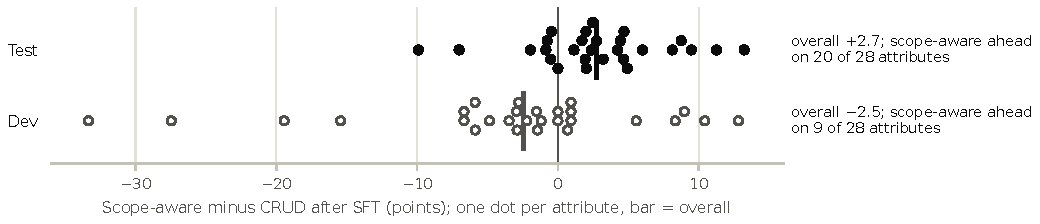
\includegraphics[width=\textwidth]{figures/report_fig_attributes.pdf}
\caption{Scope-aware minus CRUD after SFT for each of the 28 attributes of test and of dev (post-hoc). The splits share no attribute.}
\label{fig:attributes}
\end{figure*}

\section{Larger reader}\label{app:bigreader}
The larger reader is Qwen3-30B-A3B-Instruct-2507 (revision \texttt{0d7cf239}, every file's size and hash pinned in the repository), run with prompt version 3, greedy decoding, the 160-token budget and batch size 64. Since all 80\,GB GPUs of the cluster were busy, each job used two 48\,GB GPUs with the first 24 decoder layers (plus embeddings, final norm and output layer) on one and the other 24 on the other. The first attempt let the \texttt{accelerate} library place the layers; every reply was garbage and none had the ``Answer:'' line. A check job showed that on these nodes all 40 direct GPU-to-GPU copies of random tensors differed from the source although the driver reported peer access, while all 20 copies through host memory were exact. We therefore copy every tensor that crosses between the GPUs through host memory, and replace the library's loop over the experts of each mixture-of-experts block by the same loop with the routing sorted once per layer; outputs were bit-identical on the tested layers and 24 greedy tokens. Checks confirmed that only the reader differs from the 4B runs (same episodes, memories and prompts) and that every probe was answered once per condition (24,570 answers on dev, 47,103 on test and the challenge set). The re-reads took 21 hours of two-GPU jobs.

\section{Manual error analysis}\label{app:manual}
\todo{Fill in after labelling: settled counts per source and arm, raw agreement and kappa.}
The sample was fixed before the test split was read: \texttt{analysis error-sample} on the SFT seed-0 test run, 40 wrong probes per arm drawn with seed 0. Each packet item shows the question, options, gold answer, the Answer Agent's reply, the arm's memory and the gold memory at the probe, and every event up to the probe with its gold and predicted output. Two annotators label each item alone with the first applicable source: \emph{data} (the question, options or gold answer is wrong or ambiguous), \emph{executor rejection} (a rejected output held the needed write), \emph{action} (a wrong, missing or spurious accepted write), \emph{reader matching} (the memory is right but its words do not plainly match the question or options), \emph{answer reasoning} (the memory is right and plainly matches, and the reader still chooses wrong), or \emph{other}; disagreements are settled by discussion.

\section{Reproducibility}\label{app:repro}
Settings were frozen under the git tag \texttt{freeze-p12}. SHA-256 prefixes: data train \texttt{494b76c7}, dev \texttt{c8bd3dea}, test \texttt{f5e680a1}, challenge set \texttt{ffeb6a87}; policy instructions scope-aware \texttt{a41fed14}, CRUD \texttt{6d54c95c}; SFT rows \texttt{beaca8bd} and \texttt{e5745306}. The repository contains the protocol and executors (\texttt{scope\_memory/protocol.py}), the evaluator (\texttt{evaluate.py}), the analyses (\texttt{analysis.py}, \texttt{posthoc.py}, \texttt{readtime.py}), the cluster scripts (\texttt{training/sft/}), the result files behind every table (\texttt{results/}) and the annotation packets (\texttt{annotations/}).

\end{document}
